\graphicspath{{./Sturm_Liouville/}}

\section{Sturm Liouville Theory and Orthonogal Expansions!}

Sturm-Liouville theory regards second-order linear differential equations of the form

\begin{equation}
\label{SL_eq} \frac{d}{dx} \left[ p(x) \frac{dy}{dx} \right] + q(x) y = -\lambda w(x) y,
\end{equation} 

where $p(x), q(x)$, and $w(x)$ are  all continuous functions on the particular region of interest, say $[a,b]$. We also note that $w(x)>0$ and is referred to as the ``weight" function as well as that we assume $p(x)\in C^n$ with $n\geq 1$.\\

We further note that in this formalism we consider the solution $y(x)$ to obey boundary conditions on $[a,b]$. Moreover $\lambda$ is an eigenvalue of the our Sturm-Liouville operator and is chosen to give non-trivial solutions of (\ref{SL_eq}), which satisfy the boundary conditions.   \\

What makes Sturm-Liouville theory interesting and of particular use in applied mathematics is the factor that the linear differential operator given by (\ref{SL_eq}) is \emph{Hermitian} in some function space for specific boundary conditions.  What is special about \emph{Hermitian} operators is that their eigenfunctions are orthogonal (sometimes with the assistance of a weight function, i.e., $w(x)$) and form a complete function space. Recall how Hermitian operators work in Linear Algebra - they lead to a basis of orthogonal eigenvectors, each with real associated eigenvalue. \\


\begin{theorem}
\label{SL_theorem} If a Sturm-Liouville problem is \emph{regular}, i.e., if $p(x), p'(x), q(x),$ and $w(x)$ are all continuous on $[a,b]$ and have boundary conditions that can be written as 
\begin{align}
\label{SL_bcs} \alpha_1 y(a) + \alpha_2 y'(a) &= 0 \ \ \ \ \ \ with \ \ \ \ \ \alpha_1^2+\alpha^2>0 \\
\beta_1 y(b) + \beta_2 y'(b) &= 0 \ \ \ \ \ \ with \ \ \ \ \ \beta_1^2+\beta^2>0, 
\end{align}

then the eigenvalues of the Sturm-Liouville problem are real and can be ordered such that
$$\lambda_1 < \lambda_2 < \lambda_3 < \cdots < \lambda_n < \cdots \rightarrow \infty.$$
Furthermore with each eigenvalue, $\lambda_j$, there is a unique eigenfunction, $\phi_j(x)$, which has exactly $(j-1)$ roots in $(a,b)$, and with orthogonality property, i.e., 
$$\int_a^b \phi_j(x) \phi_k(x) w(x) dx =\left\{ \begin{array}{c} 
1,  \ \ \ \ j=k \\
0, \ \ \ \ j\neq k \end{array} \right.$$
\end{theorem}


\subsection{Application: Fourier Series and Orthogonal Series Expansions}

In this subsection we will explore where Fourier Series comes from, as well as, how to write an arbitrary continuous function, $f(x)$, in terms of Fourier Series. 

\subsubsection{Example: Fourier Sine Series}

Consider the following BVP, 
\begin{align}
y'' + \lambda y &= 0 \\ 
y(0) &= 0 \\
y(1) & = 0.
\end{align}

Now we have three cases to consider:
\begin{enumerate}
\item $\lambda = 0$
\item $\lambda = -\alpha^2 < 0$
\item $\lambda = \alpha^2 > 0$
\end{enumerate}

\begin{itemize}
\item[Case 1: ] $\lambda = 0$: We have the following ODE to solve $$y'' = 0$$ and hence we obtain $$y(x) = c_1 + c_2 x.$$
Inserting the boundary conditions, we see that $c_1 = c_2 = 0$, and hence we only have the trivial solution in this case. 

\item[Case 2: ] $\lambda = -\alpha^2 < 0:$ We have the following ODE to solve $$y'' - \alpha^2 y = 0.$$  We find the general solution of $$y(x) = c_1 \sinh(\alpha x) + c_2 \cosh(\alpha x).$$

Using the boundary conditions we see
\begin{align*}
y(0)=0 &\Rightarrow c_2 = 0 \\
y(1)=0 &\Rightarrow c_1 \sinh(\alpha) = 0 \Rightarrow c_1 = 0. 
\end{align*}

Hence we only have the trivial solution, once again.

\item[Case 3: ] $\lambda = \alpha^2 > 0$: We consider the following ODE, $$y''+\alpha^2 y= 0,$$ where $\alpha^2>0$. We find the general solution to be

$$y(x) = c_1 \sin(\alpha x) + c_2 \cos(\alpha x).$$

Using the boundary conditions we see
\begin{align*}
y(0)=0 &\Rightarrow c_2 = 0 \\
y(1)=0 &\Rightarrow c_1 \sin(\alpha) = 0 \Rightarrow \alpha = n\pi \ \ \ \mbox{where}\ n\in\mathbb{Z}^{+}. 
\end{align*}

Therefore we find our eigenvalues to be $\lambda_n = \alpha_n^2 = n^2\pi^2,$ for $n\in\mathbb{Z}^{+}$, with associated eigenfunctions, $\phi_n(x) = \sin(n\pi x).$
%


We will now demonstrate the orthogonality of those eigenfunctions.

\item[Orthogonality: ]

Consider $$\int_0^1 \sin(n\pi x) \sin(m \pi x) dx,$$

where $n\neq m.$ Now we use the following identity to perform the integration,

$$\sin(a)\sin(b) = \frac{1}{2} \Big[ \cos(a-b) - \cos(a+b) \Big].$$

\begin{align*}
\int_0^1 \sin(n\pi x) \sin(m \pi x) dx &= \int_0^1   \frac{1}{2} \Big[ \cos( (n-m)\pi x) - \cos( (n+m)\pi x) \Big]  dx \\
%
&= \frac{1}{2} \Big[ \frac{1}{(n-m)\pi}  \sin( (n-m)\pi x) - \frac{1}{(n+m)\pi}  \sin( (n+m)\pi x)  \Big]_0^1 \\
%
&= 0.
\end{align*}

We note that the case $n=m$ must be considered by itself, to avoid singularity in the above integration. Moreover, the case where $n=m=0$ is disgarded since $0$ is not an eigenvalue of the differential operator. Now we show the case $n=m\neq 0$ leads to a non-zero computation. 

Now considering $n=m\neq 0$,

\begin{align*}
\int_0^1 \sin^2(n\pi x)dx &= \frac{1}{2} \int_0^1\Big[1 - \cos(2n\pi x)\Big] dx \\
%
&= \frac{1}{2} \Big[x - \frac{1}{2n\pi} \sin(2n\pi x) ]_0^1 \\
%
&= \frac{1}{2}.
\end{align*}

Hence orthogonality holds (as it should)!

\end{itemize}


%
%
% FOURIER SERIES EXAMPLE!
%
%
\subsubsection{Example: Fourier Series of a function $f(x)$}

Now we will illustrate how to use this idea of Fourier Series in rewriting a function, $f(x)$. First we begin with the general form of a Fourier Series. Written as an infinite sum, a Fourier Series of a function $f(x)$ on an interval $[-L,L]$ is written as,

\begin{equation}
\label{fourier_series} f(x) = \sum_{j=0}^{\infty} a_j \cos\left( \frac{j\pi x}{L} \right ) +  \sum_{j=1}^{\infty} b_j \sin\left( \frac{j\pi x}{L} \right ).
\end{equation}

The brunt of the work is now calculating the coefficients $\{a_n\}_{n=0}^{\infty}$ and $\{b_n\}_{n=1}^{\infty}$. Luckily we can employ orthogonality properties of the Fourier eigenfunctions.

\begin{align}
\int_{-L}^L \cos\left( \frac{n\pi x}{L} \right ) \cos\left( \frac{m\pi x}{L}\right) dx &=\left\{\begin{array}{c}2L\ \ \ \ n=m=0 \\ L \ \ \ \ n=m>0 \\ 0 \ \ \ \ n\neq m \end{array}\right. \\
\int_{-L}^L \sin\left( \frac{n\pi x}{L} \right ) \sin\left( \frac{m\pi x}{L} \right) dx &= \left\{\begin{array}{c} L \ \ \ \ n=m>0 \\ 0 \ \ \ \ n\neq m \end{array}\right. \\
\int_{-L}^L \sin\left( \frac{n\pi x}{L} \right ) \cos\left( \frac{m\pi x}{L} \right) dx &= 0.
\end{align}

To compute the coefficients, we begin with (\ref{fourier_series}) and multiply by either eigenfunction. First let's consider the contributions by the $\Big\{  \sin\left( \frac{n\pi x}{L} \right ) \Big\}$ eigenfunctions in the expansion of $f(x)$. We begin with

$$f(x) = \sum_{n=0}^{\infty} a_n \cos\left( \frac{n\pi x}{L} \right ) +  \sum_{n=1}^{\infty} b_n \sin\left( \frac{n\pi x}{L} \right ),$$

and multiply both sides by $\sin\left( \frac{m\pi x}{L} \right )$. Next we integrate both sides over the interval of interest, e.g.,

$$\int_{-L}^L f(x) \sin\left( \frac{m\pi x}{L} \right )  dx=\int_{-L}^{L}\Bigg[ \sum_{n=0}^{\infty} a_n \cos\left( \frac{n\pi x}{L} \right ) +  \sum_{n=1}^{\infty} b_n \sin\left( \frac{n\pi x}{L} \right ) \Bigg] \sin\left( \frac{m\pi x}{L} \right ) dx.$$

The only terms that are not zero in the above equation, are those for which $n=m$ and the sinusoidal terms, i.e.,

$$\int_{-L}^L f(x) \sin\left( \frac{m\pi x}{L} \right )  dx = \int_{-L}^{L} b_m \sin^2\left( \frac{m\pi x}{L} \right ) dx.$$

Hence since $b_m$ is a constant, we can solve for it to get

$$b_m = \frac{ \int_{-L}^L f(x) \sin\left( \frac{m\pi x}{L} \right )  dx }{  \int_{-L}^{L} \sin^2\left( \frac{m\pi x}{L} \right ) dx }.$$

Therefore we now have a formula to find all the coefficients $\{b_j\}_{j=1}^{\infty}.$ Using a similar approach and employing orthogonality once again, we can find a formula for the $\{a_j\}_{j=0}^{\infty}$ coefficients as well, i.e., 

$$a_m = \frac{ \int_{-L}^L f(x) \cos\left( \frac{m\pi x}{L} \right )  dx }{  \int_{-L}^{L} \cos^2\left( \frac{m\pi x}{L} \right ) dx }.$$

After computing all those integrals, we will have our expansion of $f(x)$ on $[-L,L]$ in all its Fourier Series glory!


%
%
% FOURIER SERIES OF f(x) = x
%
%
\subsubsection{Example: Fourier Series of $f(x)=x$ on $[-\pi,\pi]$}

We wish to find $$f(x) = x = \sum_{j=0}^{\infty} a_j \cos(jx)+  \sum_{j=1}^{\infty} b_j \sin(jx).$$

Welp, let's do the integrals!

\begin{align*}
b_m &= \frac{ \int_{-\pi}^{\pi} x \sin(mx) dx }{  \int_{-\pi}^{\pi} \sin^2(mx) dx }. \\
&= \frac{ -\frac{x}{m}\cos(mx) \Big|_{-\pi}^{\pi} + \frac{1}{m}\int_{-\pi}^{\pi} \cos(mx) dx }{\pi} \\
&= \frac{ \frac{-2\pi}{m} cos(m\pi) }{\pi} \\
& = \frac{2}{m} (-1)^{m+1}
\end{align*}

Similarly, we'll consider the integrations to find $\{ a_n \}$. Let's start with $m>0$,
\begin{align*}
a_m &= \frac{ \int_{-\pi}^{\pi} x \cos(mx) dx }{  \int_{-\pi}^{\pi} \cos^2(mx) dx }. \\
&= \frac{ \frac{x}{m}\sin(mx) \Big|_{-\pi}^{\pi} - \frac{1}{m}\int_{-\pi}^{\pi} \sin(mx) dx }{\pi} \\
&= 0
\end{align*}

and when $m=0$ for $a_0$,

$$a_0 = \frac{ \int_{-\pi}^{\pi} x dx }{ \int_{-\pi}^{\pi} 1 dx } = 0.$$

Therefore all the cosines drop out of our Fourier Expansion of $f(x)=x$ on $[-\pi,\pi].$ Note, we could have easily seen this by the fact the function we are rewriting in the Fourier basis, $f(x)=x$, is odd on a symmetric interval.  We then have

$$f(x) = x = \sum_{m=1}^{\infty} \left[ \frac{2}{m} (-1)^{m+1}\right] \sin(mx).$$

The figure below shows what the Fourier Series expansion looks like on that interval for differing number of terms in the series.

\begin{center}
\begin{figure}[h!]
 	\centering
  	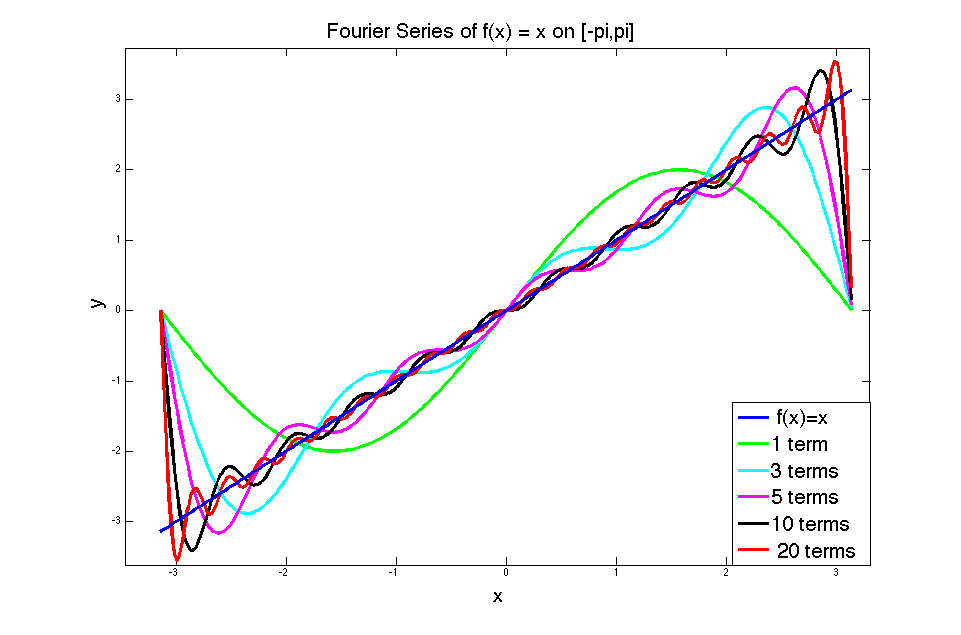
\includegraphics[scale=0.5]{Fourier_Series_Ex.png}
 	\caption{The function $f(x)=x$ being expressed as Fourier Series expansions with differing numbers of truncated terms.}
 	\label{Fourier_Series_Ex}
\end{figure}
\end{center}


%
%
% GENERAL ORTHOGONAL EXPANSIONS
%
%

\subsection{General Orthogonal Series Expansions}

As we saw in the above example, we can express a function $f(x)$ in terms of sines and cosines on a specified interval. We recall we are able to do this because the those sines and cosines, i.e., $\left\{ \cos\left( \frac{j\pi x}{L} \right ) \right\}$ and $\left\{ \cos\left( \frac{j\pi x}{L} \right ) \right\}$, on $[-L,L]$ form a complete basis in function space. Moreover, these functions were eigenfunctions of a Sturm-Liouville differential operator, so we knew we were guaranteed those properties - namely orthogonality and completeness. \\

Beyond Fourier Series there are many ``popular" orthogonal polynomials, which are all eigenfunctions of some Sturm-Liouville differential operator. Just for some buzzwords, the usual candidates tend to be:

\begin{itemize}
\item Bessel Functions
\item Chebyshev Polynomials
\item Legendre Polynomials
\item Laguerre Polynomials
\item Hermite Polynomials
\end{itemize}

More generally, if $\left\{ \phi_j(x) \right\}$ are eigenfunctions of a Sturm-Liouville problem, and we wish to expand some function $f(x)$ on an interval $[a,b]$ in terms of them, i.e., 
$$f(x) = \sum_{j=0}^{\infty} c_j \tilde{\phi}_j(x),$$

the brunt of the work still lies in calculating the coefficients $\{ c_j\}$. We note that $\tilde{\phi}_j(x)$ are the eigenfunctions, $\phi_j(x)$, just translated into the interval $[a,b].$ We can do the same procedure as we did to find the Fourier Series coefficients. Let's party!

\begin{align*}
f(x) &= \sum_{m=0}^{\infty} c_m \tilde{\phi}_m(x) \\
 f(x) \tilde{\phi}_n(x)  &=\sum_{m=0}^{\infty} c_m \tilde{\phi}_m(x) \tilde{\phi}_n(x)  \\
  f(x) \tilde{\phi}_n(x) \tilde{w}(x)  &=\sum_{m=0}^{\infty} c_m \tilde{\phi}_m(x) \tilde{\phi}_n(x) \tilde{w}(x) \\
\int_{a}^{b} f(x) \tilde{\phi}_n(x) \tilde{w}(x) dx &= \int_a^b \sum_{m=0}^{\infty} c_m \tilde{\phi}_m(x) \tilde{\phi}_n(x) \tilde{w}(x) dx \\
\int_{a}^{b} f(x) \tilde{\phi}_n(x) \tilde{w}(x) dx &= \sum_{m=0}^{\infty} c_m  \int_a^b  \tilde{\phi}_m(x) \tilde{\phi}_n(x)  \tilde{w}(x) dx \\
\int_{a}^{b} f(x) \tilde{\phi}_n(x) \tilde{w}(x) dx &=  c_n \int_a^b  \tilde{\phi}^2_n(x) \tilde{w}(x) dx \\
\end{align*}

and hence we obtain

$$c_n = \frac{  \int_{a}^{b} f(x) \tilde{\phi}_n(x) \tilde{w}(x) dx    } { \int_a^b  \tilde{\phi}^2_n(x) \tilde{w}(x) dx  }.$$

Note: $\tilde{w}(x)$ is the weight function that comes from (\ref{SL_eq}), just translated into the appropriate interval $[a,b]$.


%
%
% SOLVING ODEs WITH FOURIER SERIES!
%
%
\subsection{Using Fourier Series to Solve ODEs}

Consider the following $2^{nd}$ order linear constant-coefficient ODE:

$$\hat{L}u = \alpha u'' + \beta u' + \gamma u = g(x),$$

where $\{\alpha, \beta, \gamma\}\in\mathbb{R}$, $u=u(t)$ and and either Dirichlet, Neumann, or mixed type  boundary conditions, on some interval $[-L,L]$. If the ODE is not defined on such an interval, simply do a transformation into it. We then must solve for both the complementary solution, $u_C(x)$, i.e., the solution to the homogeneous problem, as well as the particular solution, $u_P(x)$, e.g., the solution to the non-homogeneous problem. Our full solution will be of the form $$u(x) = u_C(x) + u_P(x).$$

Now in doing the above we will employ the services of Fourier Series to find the particular solution, $u_P(x).$ We note that if $g(x)$ is a fairly simple function, e.g., a polynomial, sine, cosine, or exponential, or even products of them, finding the particular solution using \emph{undetermined coefficients} is probably the road more traveled (and it should be). If $g(x)$ is not a simple function like those, you can try to use \emph{variation of parameters}; however, if you do not know the complementary solutions, this could prove rather difficult. Now if $g(x)$ is periodic with period $2L$, this is where Fourier Series can come in!

 We wish to write our solution $u_P(x)$ in a Fourier Series, 

$$u_P(x) =  \sum_{j=0}^{\infty} a_j \cos\left( \frac{j\pi x}{L} \right ) +  \sum_{j=1}^{\infty} b_j \sin\left( \frac{j\pi x}{L} \right ).$$

However, first we must also expand $g(x)$ in its Fourier Series, e.g.,

$$g(x) =  \sum_{j=0}^{\infty} c_j \cos\left( \frac{j\pi x}{L} \right ) +  \sum_{j=1}^{\infty} d_j \sin\left( \frac{j\pi x}{L} \right );$$

however, since $g(x)$ is a known function we can find the coefficients $\{ c_j \}$ and $\{ d_j \}$ explicitly using the methods above. We now have a  linear differential equation of the form,

$$\hat{L}u = \sum_{j=0}^{\infty} c_j \cos\left( \frac{j\pi x}{L} \right ) +  \sum_{j=1}^{\infty} d_j \sin\left( \frac{j\pi x}{L} \right ).$$

Substituting our solution ansatz (the Fourier Series for $x_P(x)$) into the equation above, we see we get

\begin{align*}
\hat{L}u &= g(x) \\ \\
\hat{L}u &= \sum_{j=0}^{\infty} c_j \cos\left( \frac{j\pi x}{L} \right ) +  \sum_{j=1}^{\infty} d_j \sin\left( \frac{j\pi x}{L} \right ) \\ \\
\hat{L} \left[   \sum_{j=0}^{\infty} a_j \cos\left( \frac{j\pi x}{L} \right ) +  \sum_{j=1}^{\infty} b_j \sin\left( \frac{j\pi x}{L} \right ) \right]  &= \sum_{j=0}^{\infty} c_j \cos\left( \frac{j\pi x}{L} \right ) +  \sum_{j=1}^{\infty} d_j \sin\left( \frac{j\pi x}{L} \right ) \\ \\
 \sum_{j=0}^{\infty} a_j \hat{L} \left[ \cos\left( \frac{j\pi x}{L} \right ) \right] + \sum_{j=1}^{\infty} b_j \hat{L}\left[ \sin\left( \frac{j\pi x}{L} \right ) \right] &= \sum_{j=0}^{\infty} c_j \cos\left( \frac{j\pi x}{L} \right ) +  \sum_{j=1}^{\infty} d_j \sin\left( \frac{j\pi x}{L} \right ) \\ 
\end{align*}


What is left is to write a system of equations for all the $\{a_j\}$ and $\{b_j\}$ coefficients in terms of $\{ c_j\}$ and $\{d_j\}$. Note that if the damping term in not present in the ODE, i.e., $\beta=0$, there is the possibility of the presence of resonance, so the corresponding frequency term must include a polynomial type coefficient, $i.e., x$, as well.\\  

Furthermore we note that if we have Dirichlet boundary conditions, we will use a Fourier Sine Series for both $g(x)$ and $y_P(x)$, if Neumann, we will use the Fourier Cosine Series for them. 






%%%%%%%%%%%%%%%%%%%%%%%%%%%%%%%%%%
%
%
% GRAM SCHMIDT
%
%
%%%%%%%%%%%%%%%%%%%%%%%%%%%%%%%%%%

\subsection{Gram-Schmidt Processes...for othogonal polynomials?!}

If you're ever in a situation where you need to know the first few othogonal polynomials in a particular basis family, have no fear! You can derive them using a Gram-Schmidt process. That's right - just like in linear algebra. \emph{Note} that you can derive as many as you wish using this methodology...if you have enough time and mental arithmetic fortitude. \\

Before we proceed with Gram-Schmidt for othogonal polynomials we first recall the Gram-Schmidt process for othogonalizing vectors in $\mathbb{R}^n$. Once we have reviewed this, the leap to Gram-Schmidt processes for infinitely dimensinoal functional spaces will feel like a natural extension.


%
%
% GRAM-SCHMIDT FOR VECTORS IN R^n
%
%
\subsubsection{Gram-Schmidt for vectors in $\mathbb{R}^n$}

Consider a set of m-vectors in $\mathbb{R}^n$, with $m\leq n$, $\{ {\bf{v}}_1, {\bf{v}}_2, {\bf{v}}_3, \ldots, {\bf{v}}_m\}$. In general when handed a set of vectors, they will not be orthogonal; however, we will employ the services of Gram-Schmidt to help us achieve this feat. In order for the Gram-Schmidt process to achieve a set of m-orthogonal vectors from a collection of vectors, all the vectors must be linearly independent. We note that the span of the original vector space and that of the orthogonalized vector space are equivalent. 

To orthogonalize a collection of vectors, we begin with a single vector, say ${\bf{q}}_1={\bf{v}}_1$. Next we proceed to find an orthogonal vector to ${\bf{q}}_1$, by taking ${\bf{v}}_2$ and subtracting off the projection of ${\bf{v}}_2$ onto ${\bf{q}}_1$. To find the next orthogonal vector, we will repeat this process and take ${\bf{v}}_3$ and subtract off the projections of ${\bf{v}}_3$ onto ${\bf{v}}_1$ and ${\bf{q}}_2$. This process is illustrated below.

\begin{align*}
{\bf{q}}_1 &= {\bf{v}}_1 \\ 
{\bf{q}}_2 &= {\bf{v}}_2 - proj_{ {\bf{q}}_1 } {\bf{v}}_2 \\
{\bf{q}}_3 &= {\bf{v}}_3 - proj_{ {\bf{q}}_1 } {\bf{v}}_3  - proj_{ {\bf{q}}_2} {\bf{v}}_3\\ 
{\bf{q}}_4 &= {\bf{v}}_4 - proj_{ {\bf{q}}_1 } {\bf{v}}_4  - proj_{ {\bf{q}}_2} {\bf{v}}_4 - proj_{ {\bf{q}}_3} {\bf{v}}_4 \\ 
& \vdots  \\ 
{\bf{q}}_m &=  {\bf{v}}_m - \sum_{k=1}^{m-1} proj_{ {\bf{q}}_k }   {\bf{v}}_m.
\end{align*}

We now recall the strict definition of a vector projection. The projection of a vector ${\bf{v}}$ onto a vector ${\bf{u}}$ is defined as

 $$proj_{{\bf{u}}} {\bf{v}}= \frac{< {\bf{v}} , {\bf{u}}> }{ < {\bf{u}} , {\bf{u}} >  } {\bf{u}}, $$ 

$<\cdot, \cdot>$ is an inner-product.

Hence we can rewrite the Gram-Schmidt process in terms  of inner-products, e.g.,

\begin{align*}
{\bf{q}}_1 &= {\bf{v}}_1 \\ 
{\bf{q}}_2 &= {\bf{v}}_2 -  \frac{< {\bf{v}}_2 , {\bf{q}}_1 > }{ < {\bf{q}}_1 , {\bf{q}}_1 >  } {\bf{q}}_1 \\
{\bf{q}}_3 &= {\bf{v}}_3 - \frac{< {\bf{v}}_3 , {\bf{q}}_1 > }{ < {\bf{q}}_1 , {\bf{q}}_1 >  } {\bf{q}}_1  - \frac{< {\bf{v}}_3 , {\bf{q}}_2 > }{ < {\bf{q}}_2 , {\bf{q}}_2 >  } {\bf{q}}_2\\ 
{\bf{q}}_4 &= {\bf{v}}_4 - \frac{< {\bf{v}}_4 , {\bf{q}}_1 > }{ < {\bf{q}}_1 , {\bf{q}}_1 >  } {\bf{q}}_1  -  \frac{< {\bf{v}}_4 , {\bf{q}}_2 > }{ < {\bf{q}}_2 , {\bf{q}}_2>  } {\bf{q}}_2 - \frac{< {\bf{v}}_4 , {\bf{q}}_3 > }{ < {\bf{q}}_3 , {\bf{q}}_3 >  } {\bf{q}}_3 \\ 
& \vdots  \\ 
{\bf{q}}_m &=  {\bf{v}}_m - \sum_{k=1}^{m-1}  \frac{< {\bf{v}}_m , {\bf{q}}_k > }{ < {\bf{q}}_k , {\bf{q}}_k >  } {\bf{q}}_k.
\end{align*}

The last thing we can do is normalize these newly found orthogonal vectors, $\{ {\bf{q}}_1, {\bf{q}}_2, \ldots, {\bf{q}}_m \}$, using the standard normalization procedure, e.g., 
$$\{ \hat{{\bf{q}}}_1, \hat{{\bf{q}}}_2, \ldots, \hat{{\bf{q}}}_m \} = \Bigg\{ \frac{ {\bf{q}}_1 }{|| {\bf{q}}_1 || },  \frac{ {\bf{q}}_2 }{|| {\bf{q}}_2 || }, \ldots,  \frac{ {\bf{q}}_m }{|| {\bf{q}}_m || } \Bigg\},$$

where $\hat{ {\bf{q}}}_k$ is now orthonormalized.  


%
%
% GRAM-SCHMIDT FOR POLYS
%
%
\subsubsection{Gram-Schmidt for Orthogonal Polynomials!}

We now shift gears slightly and look to the problem of creating a basis of orthogonal polynomials. We recall if two polynomials, say $p_k$ and$p_j$ are orthogonal then we have 

$$<p_k, p_j> = \int_{a}^{b} p_k(x) p_j(x) w(x) dx = \left\{ \begin{array}{c} 0 \ \ \ (j\neq k) \\ c\in\mathbb{R} \ \ \ (j=k)  \end{array} \right. ,$$
%
where $w(x)$ is a weight-function associated with the specific orthogonal polynomials behind the scenes Sturm-Liouville problem. On that note, we point out that in order to easily extend Gram-Schmidt from vectors in $\mathbb{R}^n$ to infinite dimensional function space, we need to define an inner-product. We do so accordingly,

$$<p_k, p_j> = \int_{a}^{b} p_k(x) p_j(x) w(x) dx.$$

For constructing families of orthogonal polynomials, we will use the above inner-product and see that any family of orthogonal polynomials is going to be generated by changing the weight function, $w(x)$, in the above inner-product. For examples, to construct the \emph{Legendre} polynomial basis we use $w(x)=1$, while for \emph{Chebyshev} polynomials the weight function is $w(x) = \frac{1}{\sqrt{1-x^2}}.$ We also need correct integration bounds, i.e., for both Legendre and Chebyshev polynomails we need $[a,b]=[-1,1].$\\

To construct the orthogonal basis of polynomials we proceed in a similar manner to the above, except starting off with $p_0=1$ as the zero-th order polynomial. To find $p_1(x)$, the $1^{st}$-order orthogonal polynomial, we subtract off the projection of the $1^{st}$-order monomial basis function onto $p_0(x)$ from $x$. We then continue in an analogous manner. The procedure can be seen as 

\begin{align*}
p_0(x) &= 1 \\
p_1(x) &= x - \frac{ < x, p_0>  }{ <p_0, p_0>  } p_0(x) \\
p_2(x) &= x^2 - \frac{ < x^2 , p_0>  }{ <p_0, p_0>  } p_0(x) -  \frac{ < x^2 , p_1>  }{ <p_1, p_1>  } p_1(x) \\
p_3(x) &= x^3 - \frac{ < x^3 , p_0>  }{ <p_0, p_0>  } p_0(x) -  \frac{ < x^3 , p_1>  }{ <p_1, p_1>  } p_1(x) -  \frac{ < x^3 , p_2>  }{ <p_2, p_2>  } p_2(x)  \\
&\vdots \\
p_n(x) &= x^n  - \sum_{k=0}^{n-1} \frac{ < x^n , p_k>  }{ <p_k, p_k>  } p_k(x). \\
\end{align*}

It is clear that doing this procedure is definitely not optimal, especially if you need to find $p_{10}(x)$, or even $p_3(x)$ for that matter. However, where this procedure becomes powerful is in the realm of numerical quadrature, or numerical integration. In a nutshell, in the Gaussian quadrature formulation of approximating integrals, one needs to (*gets to) choose \emph{both} the quadrature points as well as the weight coefficients. It turns out that one possible method for choosing the quadrature becomes is naturally found to be constructing a specific family of orthogonal polynomials and then finding the roots of the desired order, e.g., if we wish to find $2$ quadrature nodes, we would find the roots of $p_2(x)$.\\

 Furthermore because of the accuracy of Gaussian Quadrature compared to Newton-Cotes methods, where the only degrees of freedom are the weight coefficients, as the quadrature points are known \emph{a priori.}, one only needs to construct polynomials of modest order. The main difference between the two numerical integrations methods can be seen as having $2N$ degrees of freedom in Gaussian Quadrature, while only $N$ degrees of freedom in Newton-Cotes. These degrees of freedom have immediate consequence in eliminating lower order errors to achieve higher order accuracy.

%
%We will illustrate this with an example.
%
%\begin{itemize}
%
%\item[] {\bf{Example}}: Consider the following ODE: $y'' + 3y = x$ with $y(-\pi)=y(\pi)=0.$\\
%
%Luckily we have computed the Fourier Series for $g(x)=x$ on $[\pi,\pi]$ above, and found it to be: $$g(x) = x = \sum_{m=1}^{\infty} \left[ \frac{2}{m} (-1)^{m+1}\right] \sin(mx).$$
%
%Rolling through the rigmarole describe above we first assume a solution of the form $$u(x) = \sum_{j=0}^{\infty} a_j \cos(jx)+  \sum_{j=1}^{\infty} b_j \sin(jx).$$
%
%Substituting this into the ODE we get
%$$y''+3y =  \sum_{m=0}^{\infty} (3-m^2) a_m \cos(mx) +  \sum_{m=1}^{\infty} (3-m^2) b_m \sin(mx) =\sum_{m=1}^{\infty} \left[ \frac{2}{m} (-1)^{m+1}\right] \sin(mx) = g(x).$$
%
%and hence we need that 
%\begin{align*}
%(3-m^2) a_m &= 0  \\
%(3-m^2) b_m &= \frac{2}{m} (-1)^{m+1}. \\
%\end{align*}
%
%Therefore we get that $$b_m = \frac{2}{m(3-m^2)} (-1)^{m+1},$$
%
%and we get that our solution is: $$u(x) = \sum_{m=1}^{\infty} \left[ \frac{2}{m(3-m^2)} (-1)^{m+1} \right] \sin(mx).$$
%
%
%\end{itemize}